\subsection{Exploratory Training}
\begin{table}[H]
\centering
\caption{Accuracy and mIoU performance}
\label{tab:loss_ablation}
\begin{tabular}{l c c} % 修改 1：原本有两列数据（Accuracy 和 mIoU），加上表头共 3 列，需要改为 l c c
\toprule
Loss Function & Validation Accuracy & Validation mIoU \\
\midrule
CrossEntropy Loss & 0.8139 & 0.5733 \\ % 修改 2：修正拼写 CrossEntropy -> CrossEntropy
Dice Loss & 0.8173 & 0.5862 \\
Combined Loss & 0.8166 & 0.5919 \\ % 修改 3：修正拼写 Conbined -> Combined
\bottomrule
\end{tabular}
\end{table}

\subsubsection{Superiority of Dice Loss and Combined Loss}
As demonstrated in Table~\ref{tab:loss_ablation} and the training curves, both \textit{Dice Loss} and \textit{Combined Loss} outperform the standard \textit{Cross-Entropy Loss} by a significant margin, particularly in terms of mIoU. Specifically, Compared to the CE baseline (0.5733), Dice Loss and Combined Loss improve the mIoU by 1.29\% and 1.86\% respectively. 

The underlying reasons for this superiority are analyzed as follows:
\begin{itemize}
    \item \textbf{Class Imbalance} The Oxford-IIIT Pet dataset exhibits a severe pixel-level class imbalance, where the background pixels dominate the majority of the image, while the pet boundary pixels occupy only a tiny fraction. Standard Cross-Entropy loss treats each pixel equally, leading the gradients to be heavily dominated by the background class. Consequently, the model biases towards majority classes to achieve a high pixel accuracy while sacrificing smaller, critical structures.
    \item \textbf{Optimization of Regional Overlap} In contrast, Dice Loss is formulated based on the Dice coefficient, which directly measures the regional overlap between the prediction $P$ and ground truth $G$:
    \[
        \mathcal{L}_{\text{Dice}} = 1 - \frac{2 |P \cap G|}{|P| + |G|}
    \]
    Because the denominator normalizes the overlap by the total area of both regions, Dice Loss is immune to class scale imbalances. Focusing on the global structure of foreground objects.
\end{itemize}


\subsubsection{Trade-off Between Accuracy and mIoU: Dice Loss vs. Combined Loss}
Another worth mentioning phenomenon observed in Table~\ref{tab:loss_ablation} is that while \textit{Dice Loss} achieves a slightly higher Validation Accuracy (0.8173) than \textit{Combined Loss} (0.8166), its Validation mIoU (0.5862) is notably lower than that of the Combined Loss (0.5919). 

This instance stems from how Accuracy and mIoU weigh segmentation errors:
\begin{itemize}
    \item \textbf{The Limitation of Pure Dice Loss at Boundaries:} Dice Loss focuses entirely on maximizing the regional intersection. However, during the late stages of training from scratch, the gradient of Dice Loss can become unstable or vanish when the predicted mask highly overlaps with the target. This prevents the model from fine-tuning ambiguous boundaries or pixels with low confidence, leading to suboptimal segmentation on fine details like pet outlines, which drags down the mIoU score.
    \item \textbf{The Synergistic Effect of Combined Loss:} \textit{Combined Loss} solves this bottleneck by integrating Cross-Entropy and Dice Loss. In this formulation, Dice Loss quickly captures the global shape during the early training phase, while Cross-Entropy penalizes pixel-level misclassifications at the boundaries in the later phase. Although this strict pixel-level penalty slightly compromises the overall global Accuracy (by a negligible 0.07\%), it heavily refines boundary precision, thereby yielding the highest mIoU across all configurations.
\end{itemize}




\subsubsection{Training Dynamics(Exploratory)}
\begin{figure}[H]
    \centering
    % 第一张子图 (a)
    \begin{subfigure}[b]{0.31\textwidth}
        \centering
        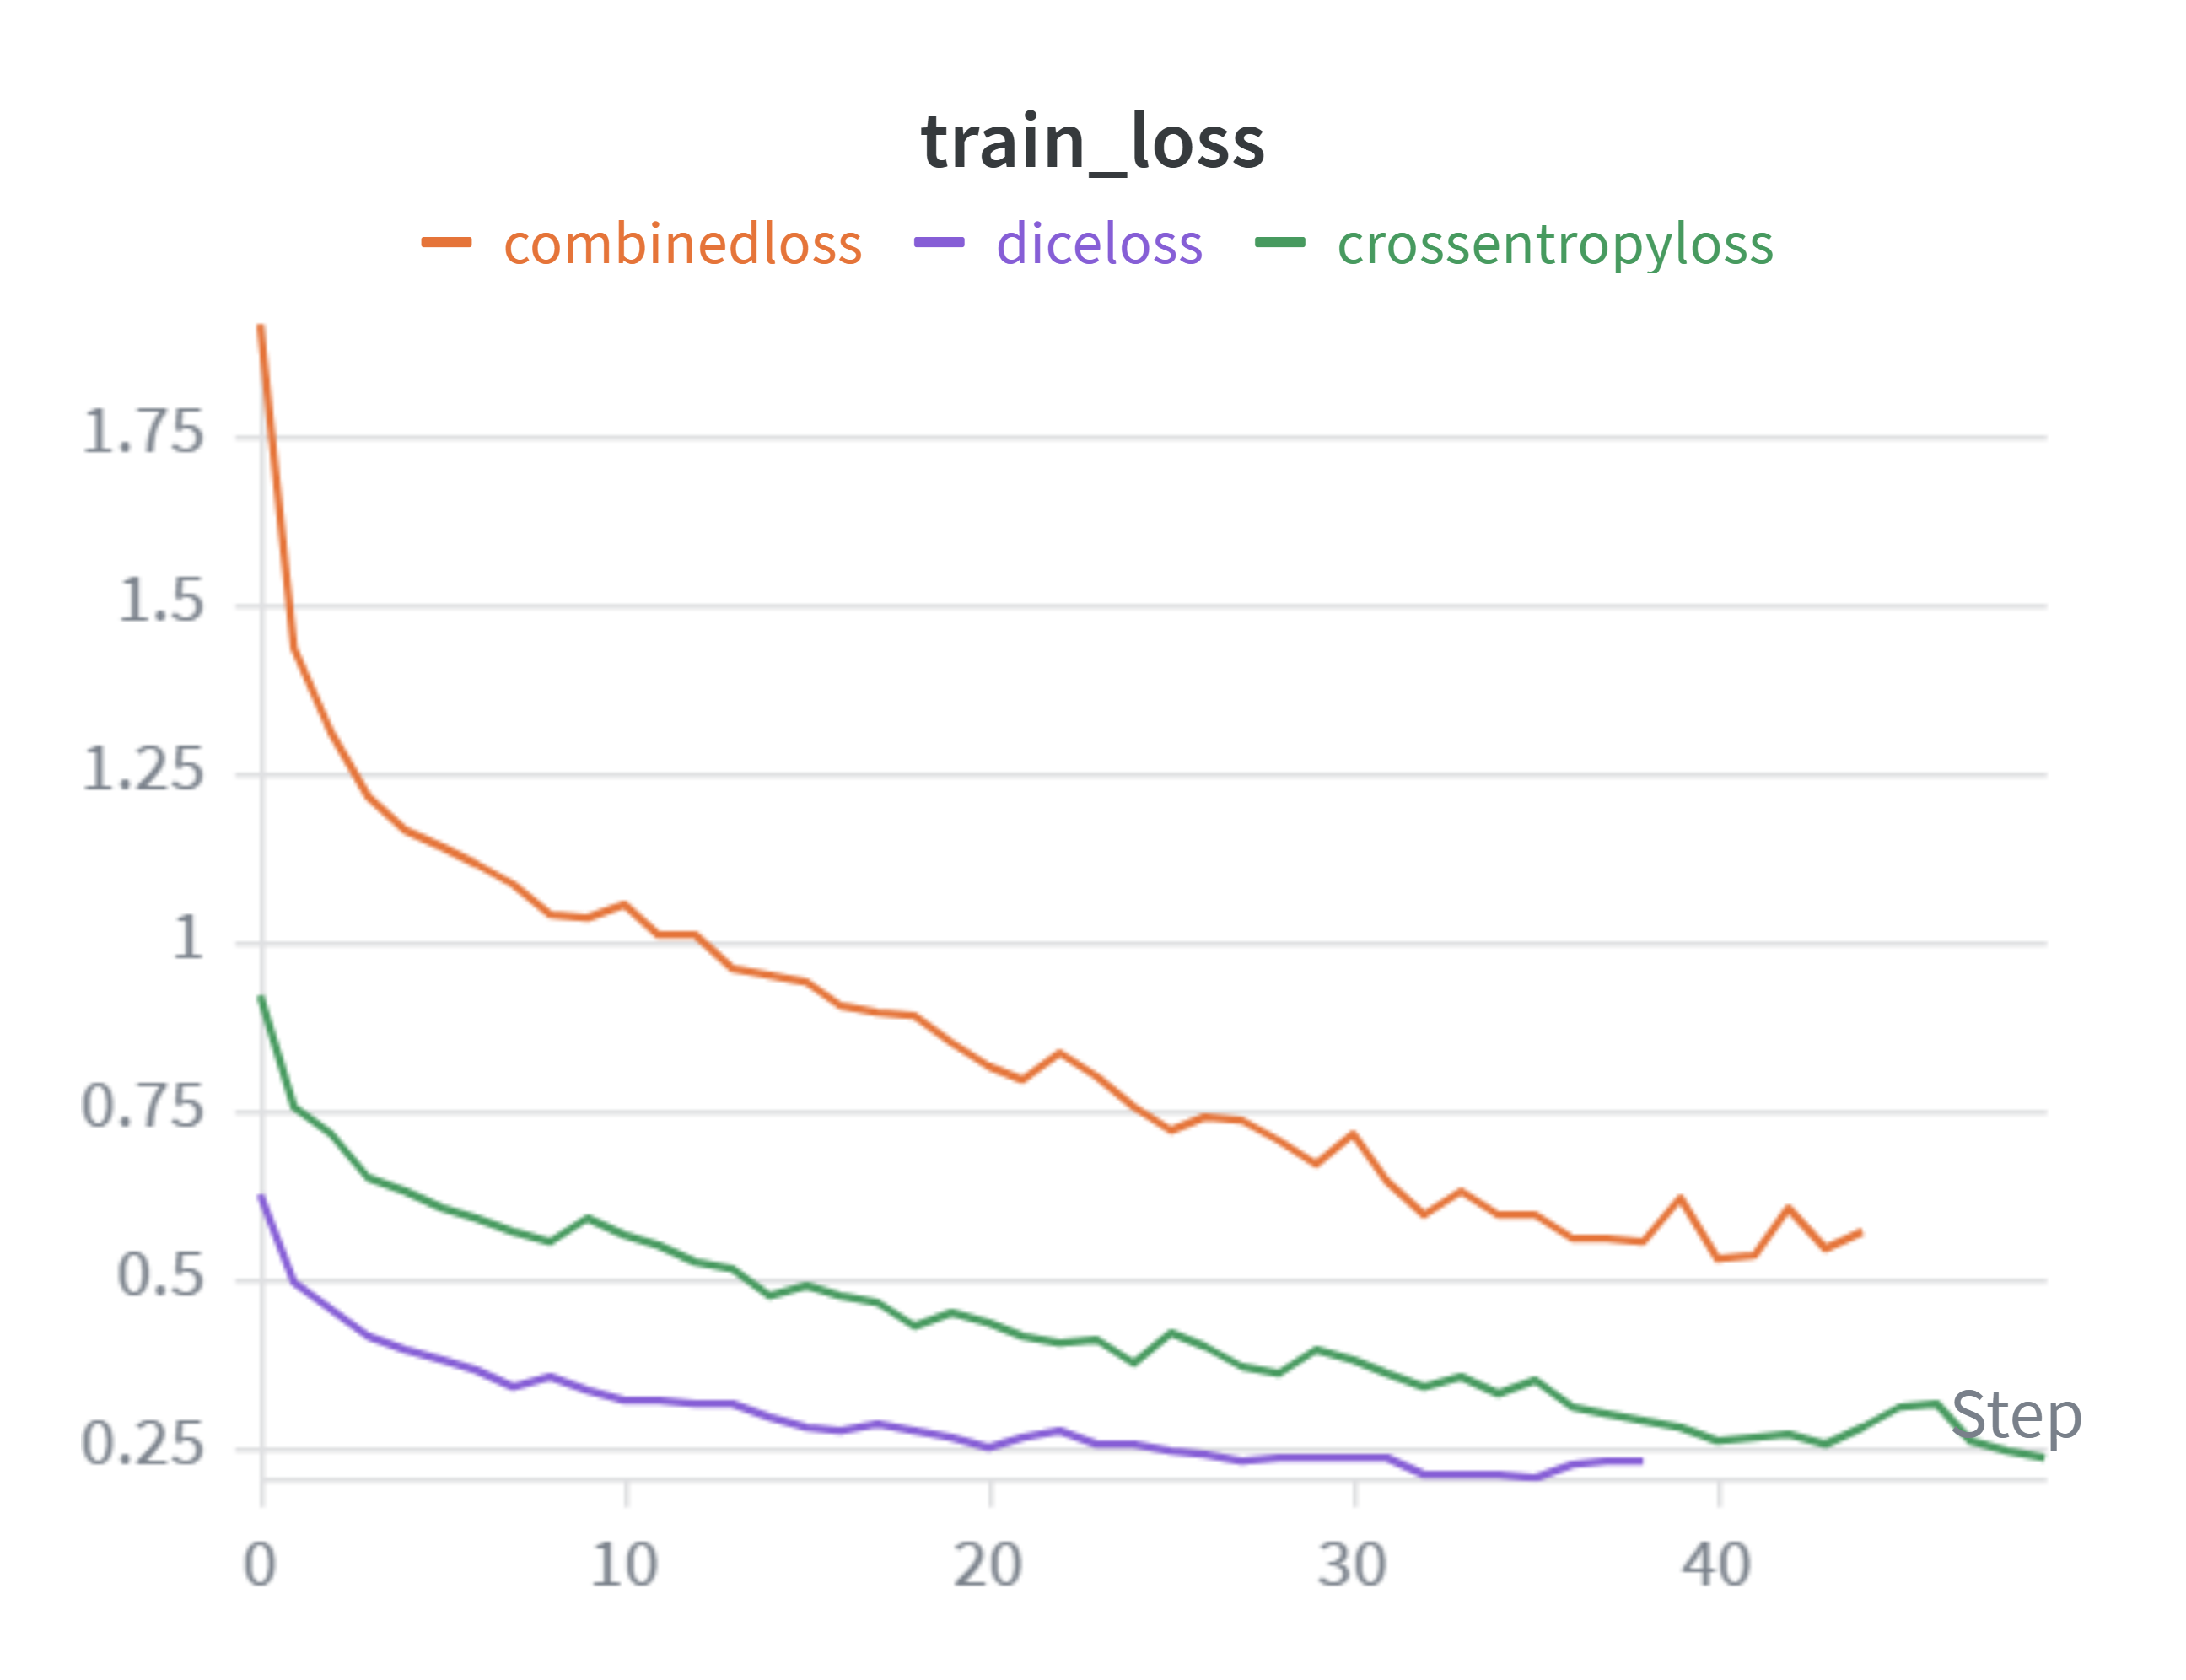
\includegraphics[width=\textwidth]{figures/task3/trainloss.png}
        \caption{Train Loss}
        \label{fig:train_loss}
    \end{subfigure}
    \hfill % 自动计算并填充子图之间的横向间距，使其两端对齐
    % 第二张子图 (b)
    \begin{subfigure}[b]{0.31\textwidth}
        \centering
        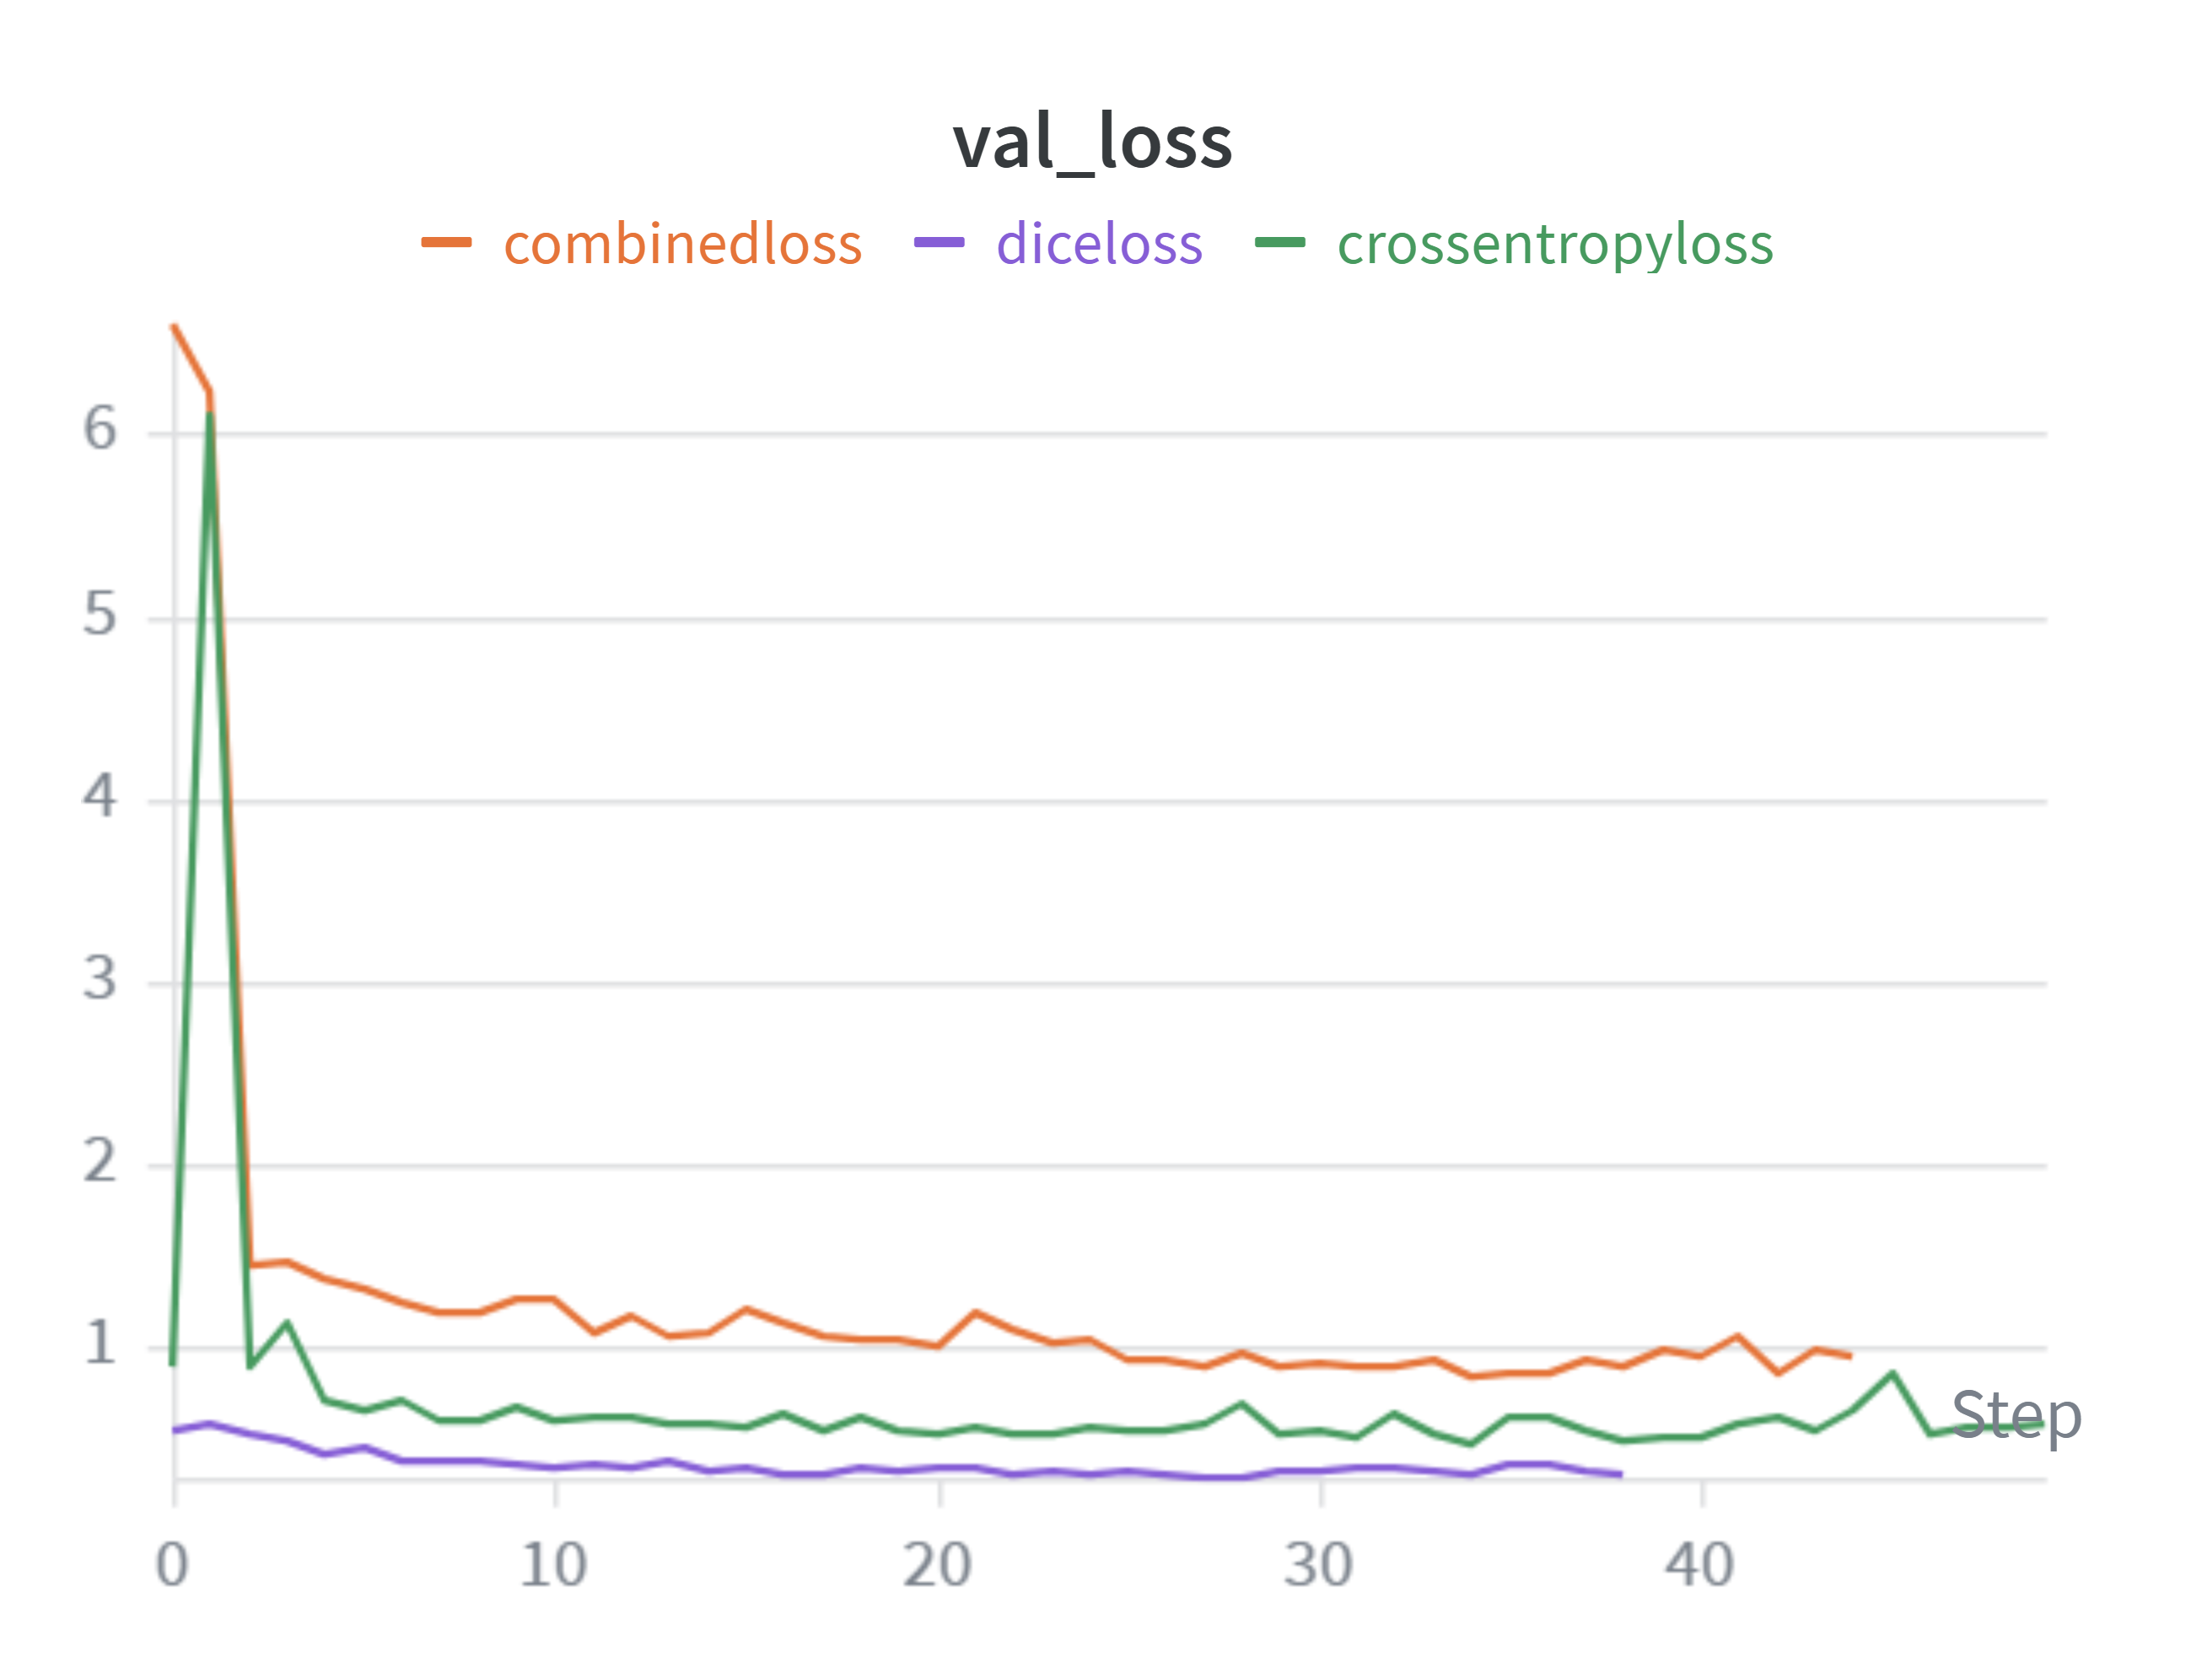
\includegraphics[width=\textwidth]{figures/task3/valloss.png}
        \caption{Val Loss}
        \label{fig:val_loss}
    \end{subfigure}
    \hfill % 自动计算并填充子图之间的横向间距
    % 第三张子图 (c)
    \begin{subfigure}[b]{0.31\textwidth}
        \centering
        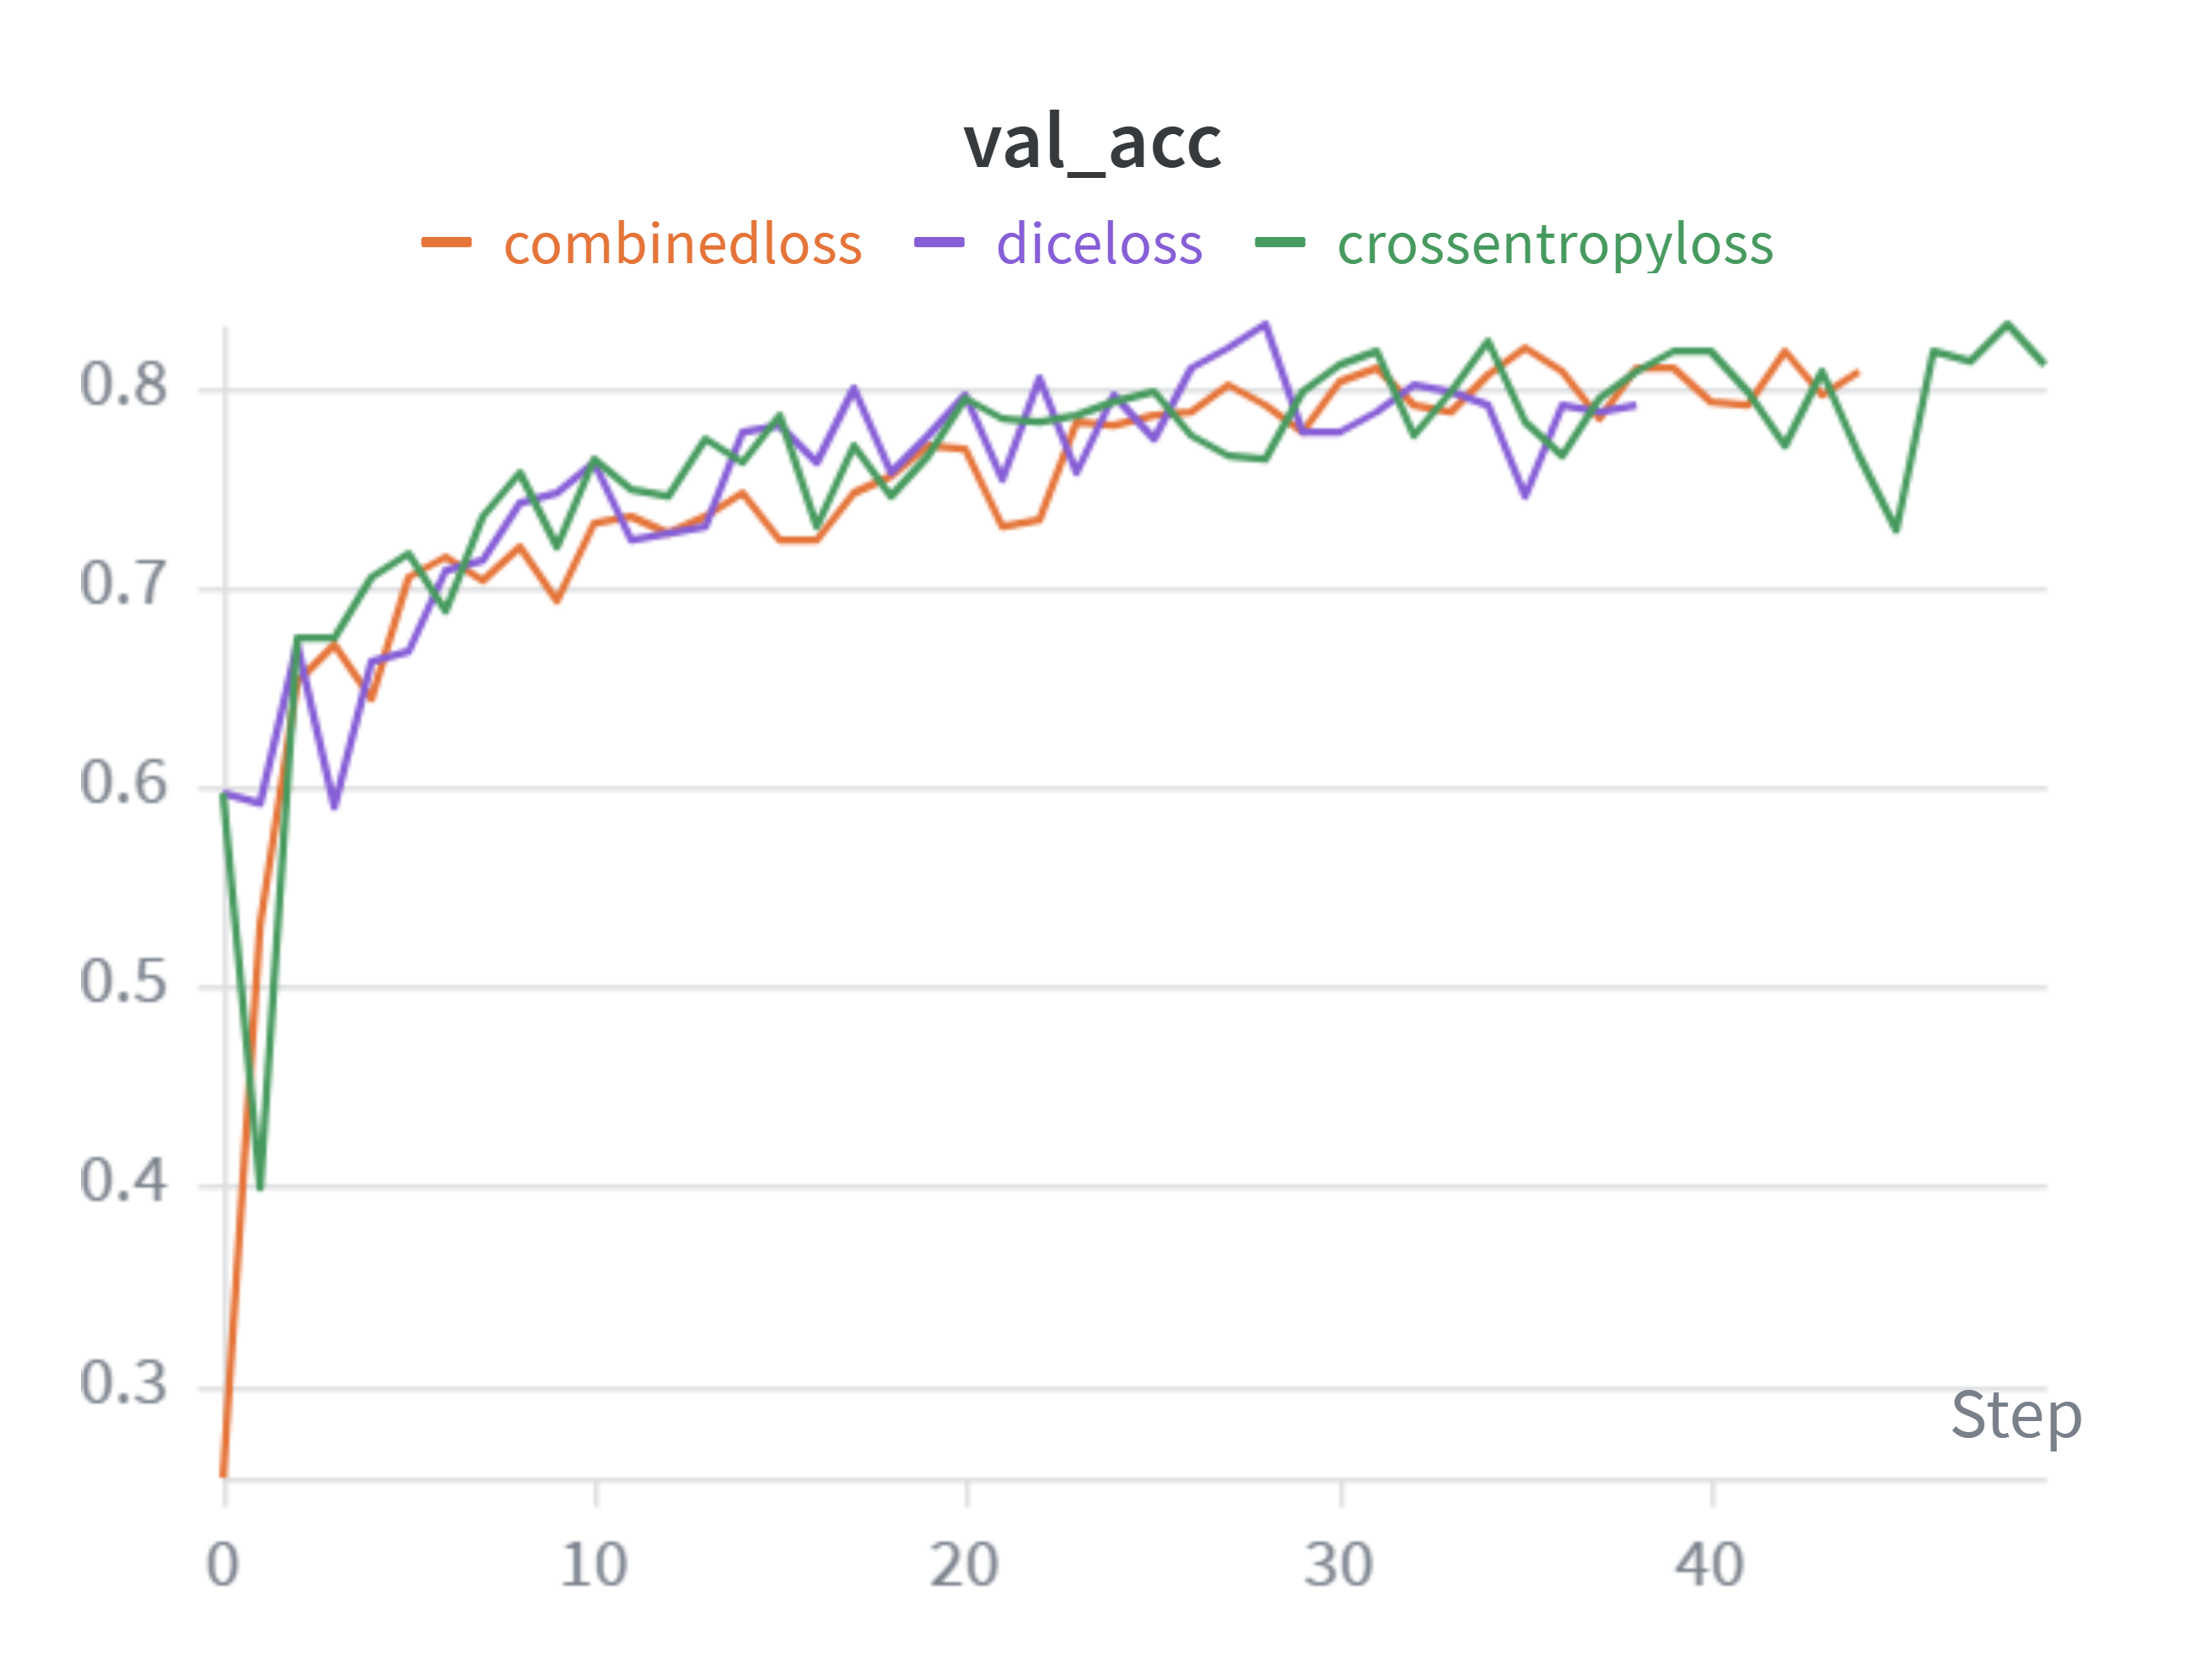
\includegraphics[width=\textwidth]{figures/task3/valaccu.png}
        \caption{Val Accuracy}
        \label{fig:val_acc}
    \end{subfigure}

    \caption{Training and validation metrics over epochs.} % 这里可以替换为你整张大图的主标题
    \label{fig:total_metrics}
\end{figure}

As is shown in the above figures, the models with different loss functions show similar optimization behavior on the training set. Their training losses decrease at comparable rates, and their training accuracies converge to nearly the same level.

Also, it's easy to see in Figure(a) that the orange curve is close to the sum of the remaining two curves, which is consistent with our definition.

It's worth mentioning that in Figure(b), the green curve(CrossEntropy Loss) has a very sharp spike at the very beginning of training (the first two steps), surging to around 6.0, before quickly dropping back and remaining stable in subsequent training sessions. While the other 2 curves have smooth overall performance with no violent fluctuations. This is because: Cross-entropy focuses on the "accuracy of pixel classification." If the model mispredicts a rare category in a large area, it will trigger a severe penalty.Dice Loss focuses on region overlap. Because it considers the sum of the predicted and ground truth regions in its denominator, it is naturally immune to pixel imbalance. Therefore, its training and validation processes are more robust and smooth.

\subsection{Final Training}
Based on our research of the exploratory experiments, we begin to analyze the final overall experimental results.
\begin{table}[H]
\centering
\caption{Accuracy and mIoU performance}
\label{tab:loss_ablation2}
\begin{tabular}{l c c} % 修改 1：原本有两列数据（Accuracy 和 mIoU），加上表头共 3 列，需要改为 l c c
\toprule
Loss Function & Validation Accuracy & Validation mIoU \\
\midrule
CrossEntropy Loss & 0.8926 & 0.7191 \\ % 修改 2：修正拼写 CrossEntropy -> CrossEntropy
Dice Loss & 0.8939 & 0.7297 \\
Combined Loss & 0.8925 & 0.7242 \\ % 修改 3：修正拼写 Conbined -> Combined
\bottomrule
\end{tabular}
\end{table}
We can similarly observe the superiority of Dice Loss and Combined Loss.

Interestingly, the trend observed in the exploratory experiments changes slightly in the final training setting. As shown in Table~\ref{tab:loss_ablation2}, Dice Loss achieves the highest Validation mIoU (0.7297), surpassing both CrossEntropy Loss and Combined Loss.

This difference can be attributed to the substantially improved training conditions in the final experiment. Compared with the exploratory stage, the final training adopts a larger batch size and a more stable optimization process, which significantly improves gradient estimation and convergence stability.

As a result, Dice Loss is able to fully exploit its region-overlap optimization objective and produce more coherent segmentation masks. Since mIoU is highly sensitive to the overlap quality between predicted and ground-truth regions, this leads to improved performance in the final training stage.

In contrast, while Combined Loss still provides stable optimization by combining pixel-wise supervision and regional overlap learning, the additional CrossEntropy component may slightly constrain the region-level optimization objective when the model has already converged well. Consequently, the performance gap between Dice Loss and Combined Loss becomes very small under the final training configuration.

\subsubsection{Training Dynamics(Final)}
\begin{figure}[H]
    \centering
    % 第一张子图 (a)
    \begin{subfigure}[b]{0.31\textwidth}
        \centering
        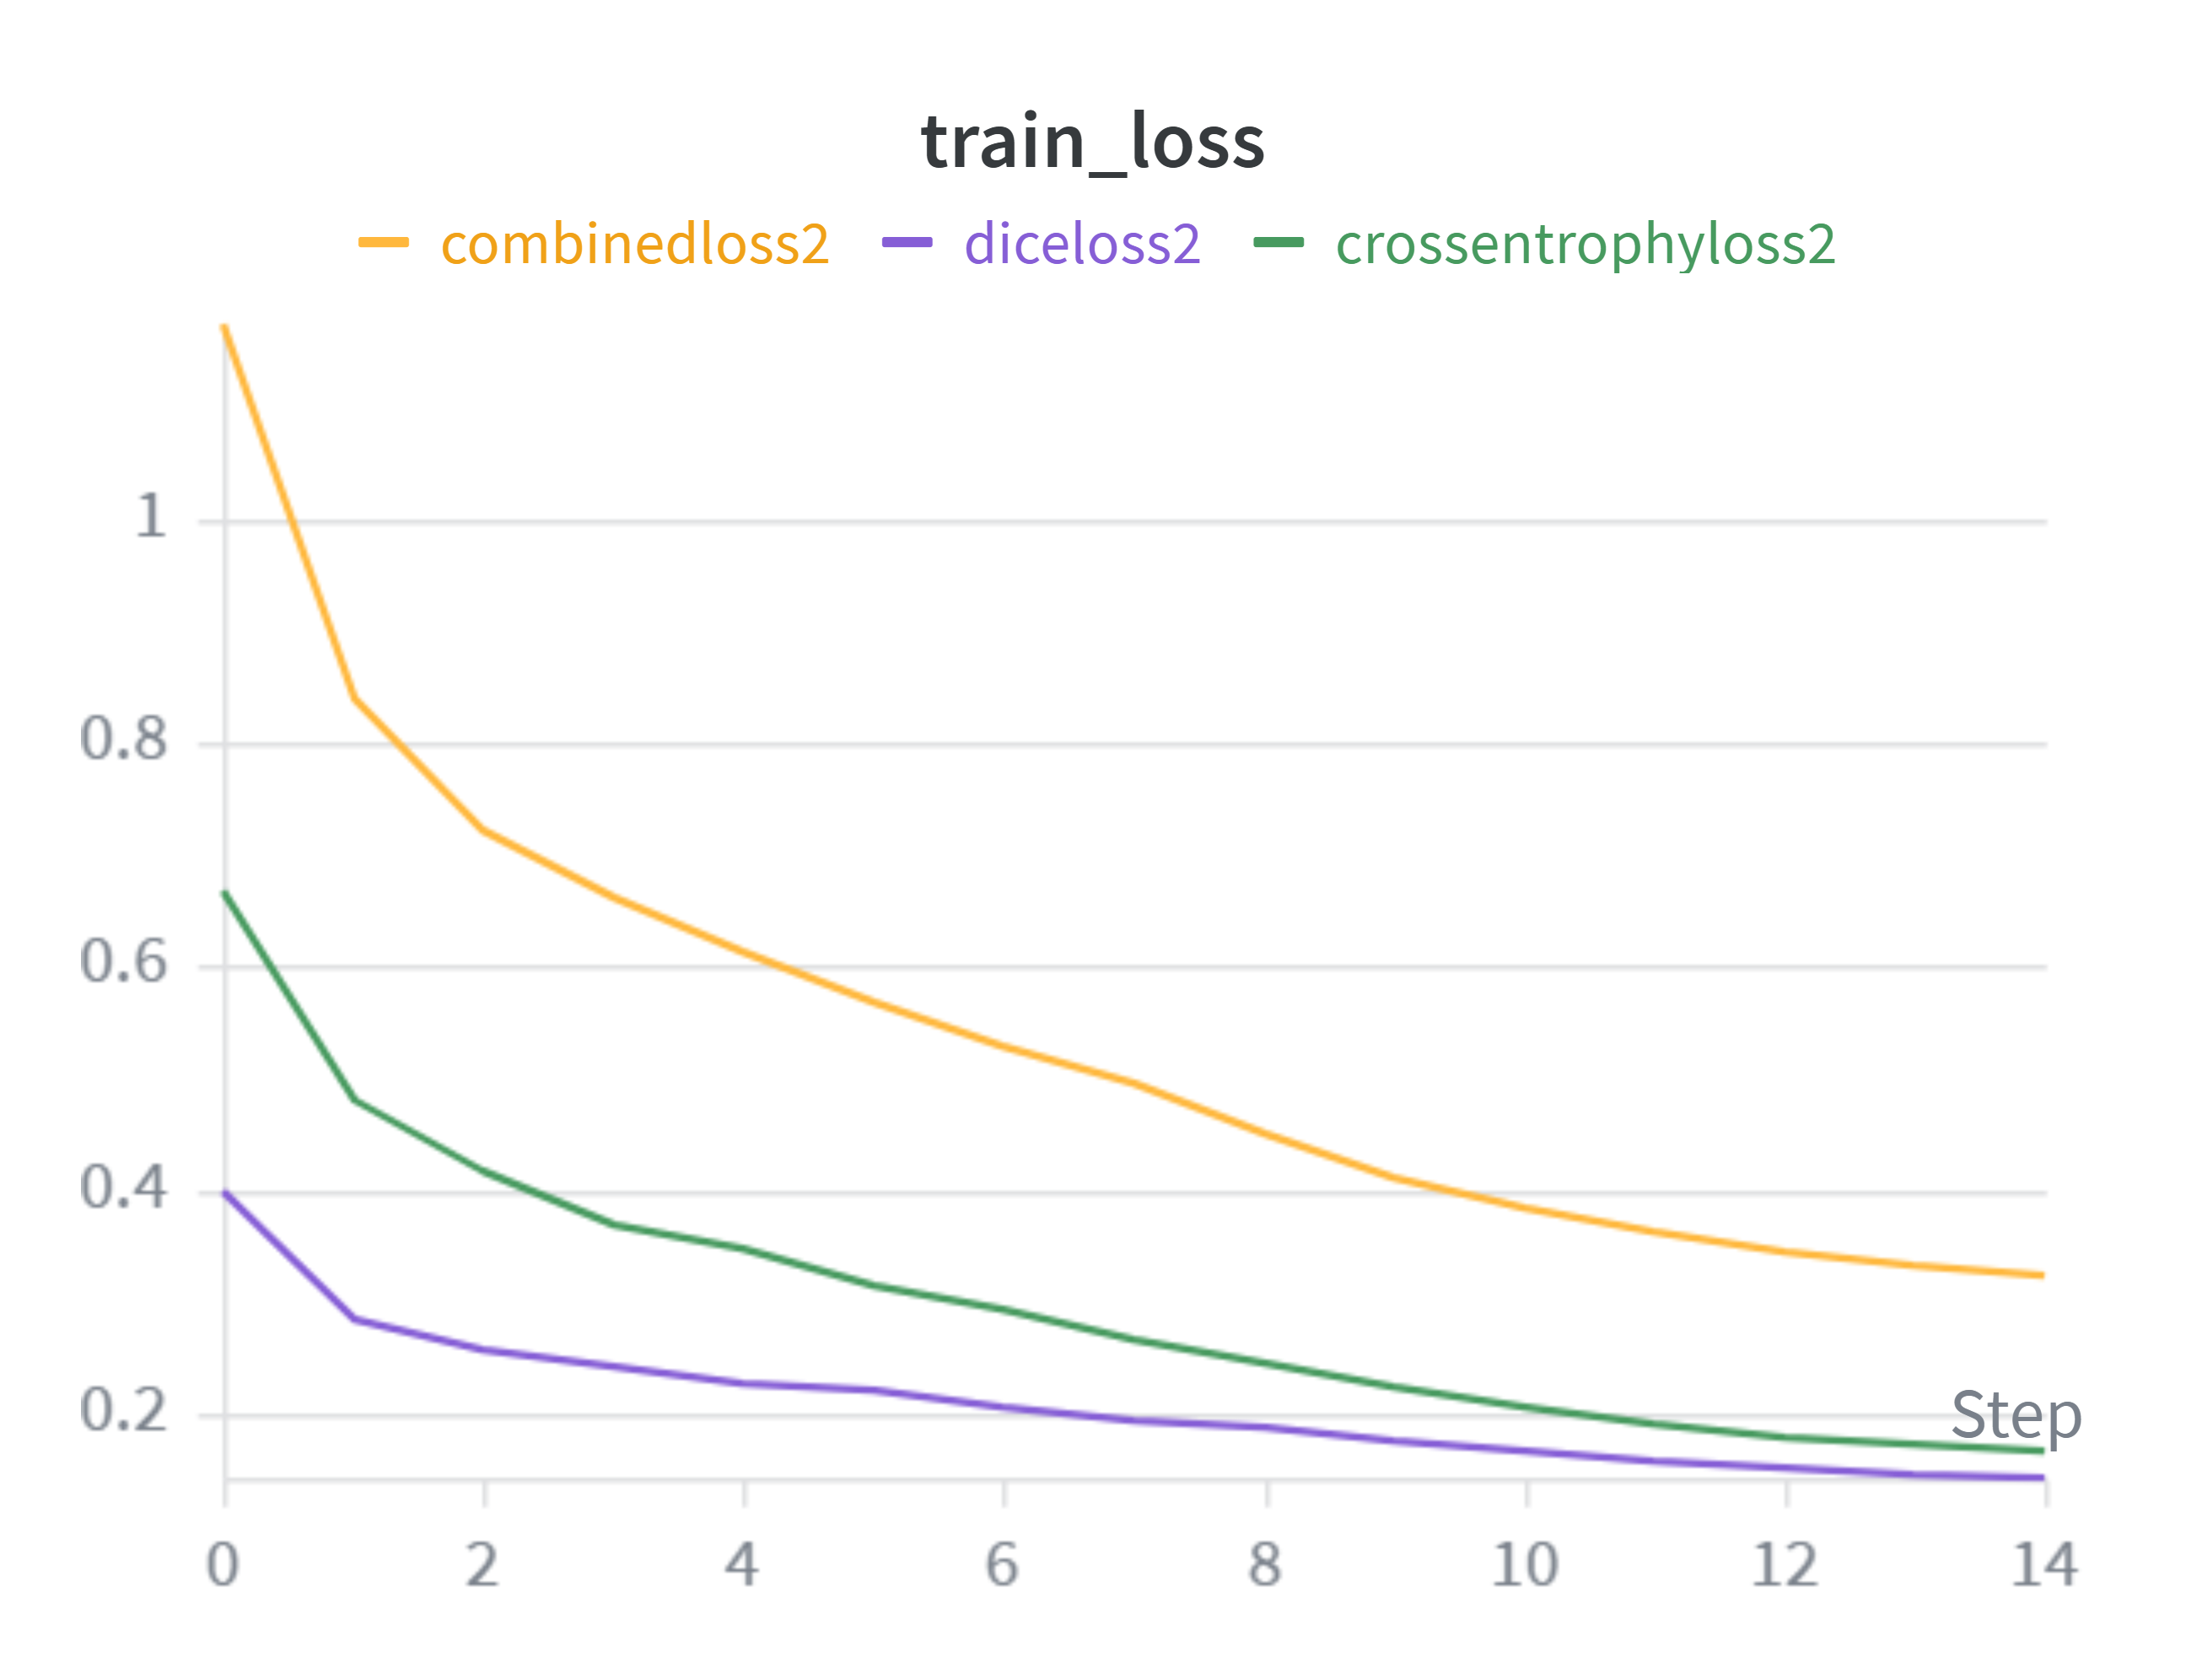
\includegraphics[width=\textwidth]{figures/task3/trainloss2.png}
        \caption{Train Loss}
        \label{fig:train_loss}
    \end{subfigure}
    \hfill % 自动计算并填充子图之间的横向间距，使其两端对齐
    % 第二张子图 (b)
    \begin{subfigure}[b]{0.31\textwidth}
        \centering
        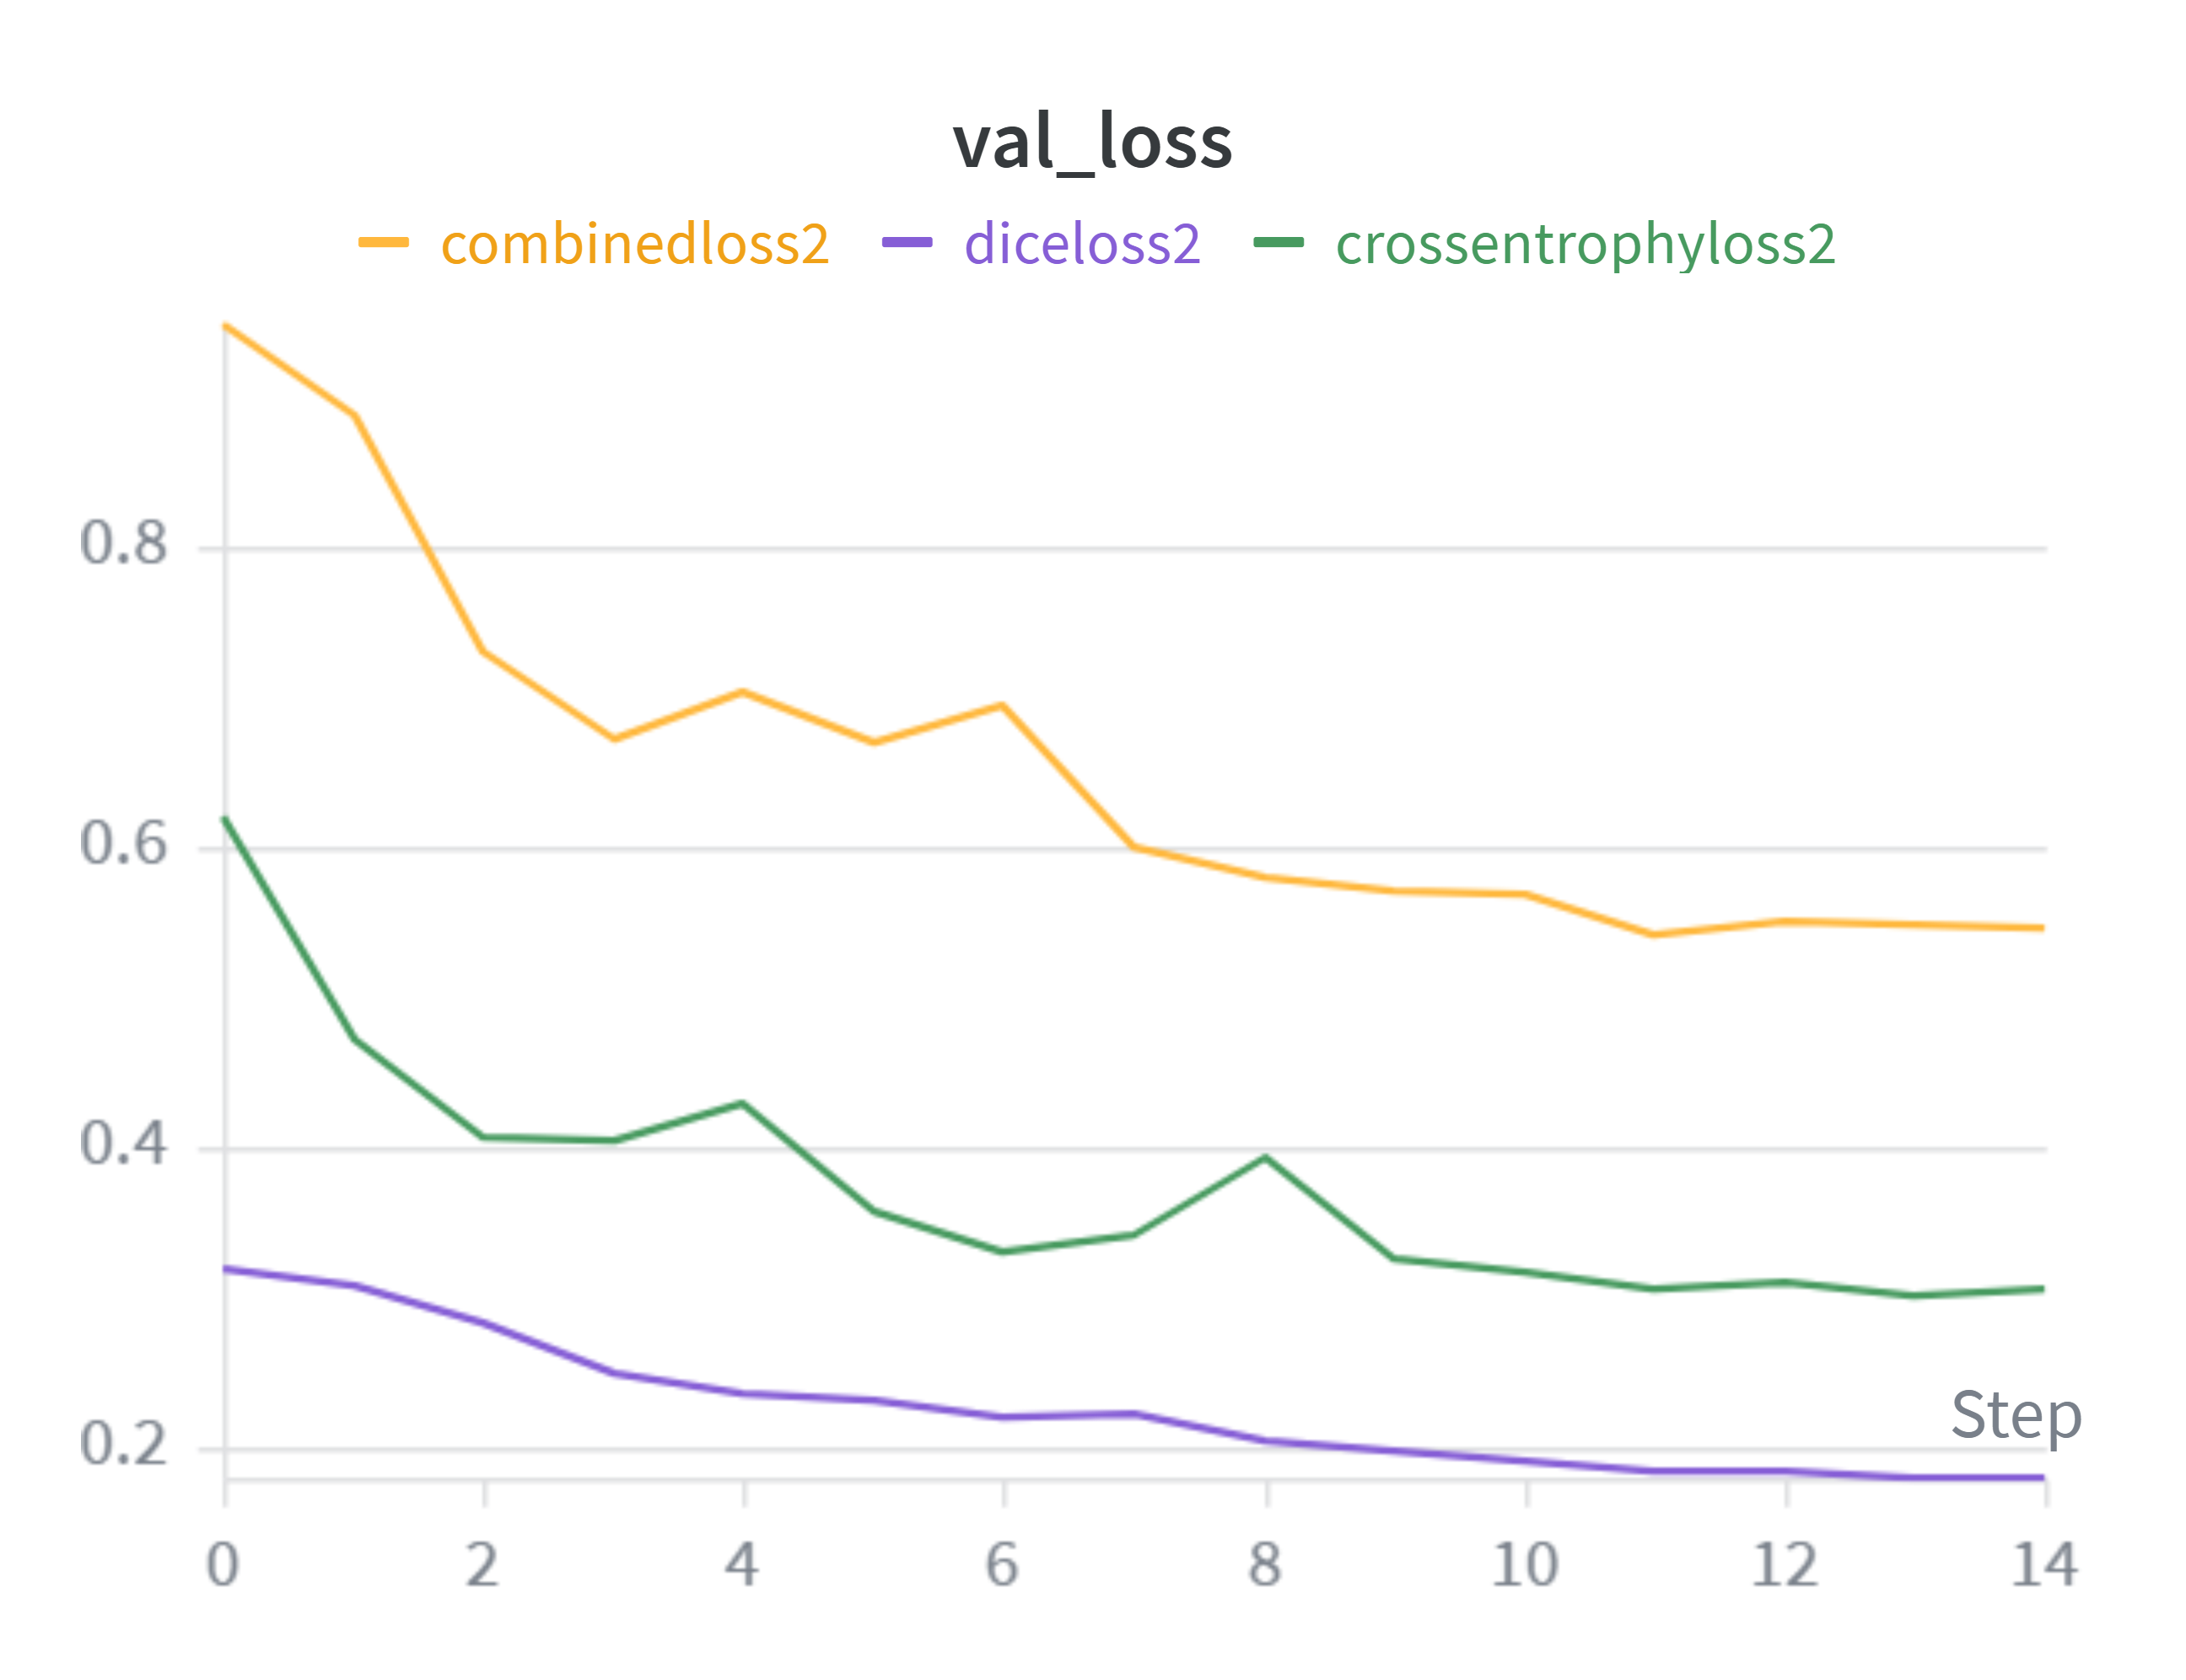
\includegraphics[width=\textwidth]{figures/task3/valloss2.png}
        \caption{Val Loss}
        \label{fig:val_loss}
    \end{subfigure}
    \hfill % 自动计算并填充子图之间的横向间距
    % 第三张子图 (c)
    \begin{subfigure}[b]{0.31\textwidth}
        \centering
        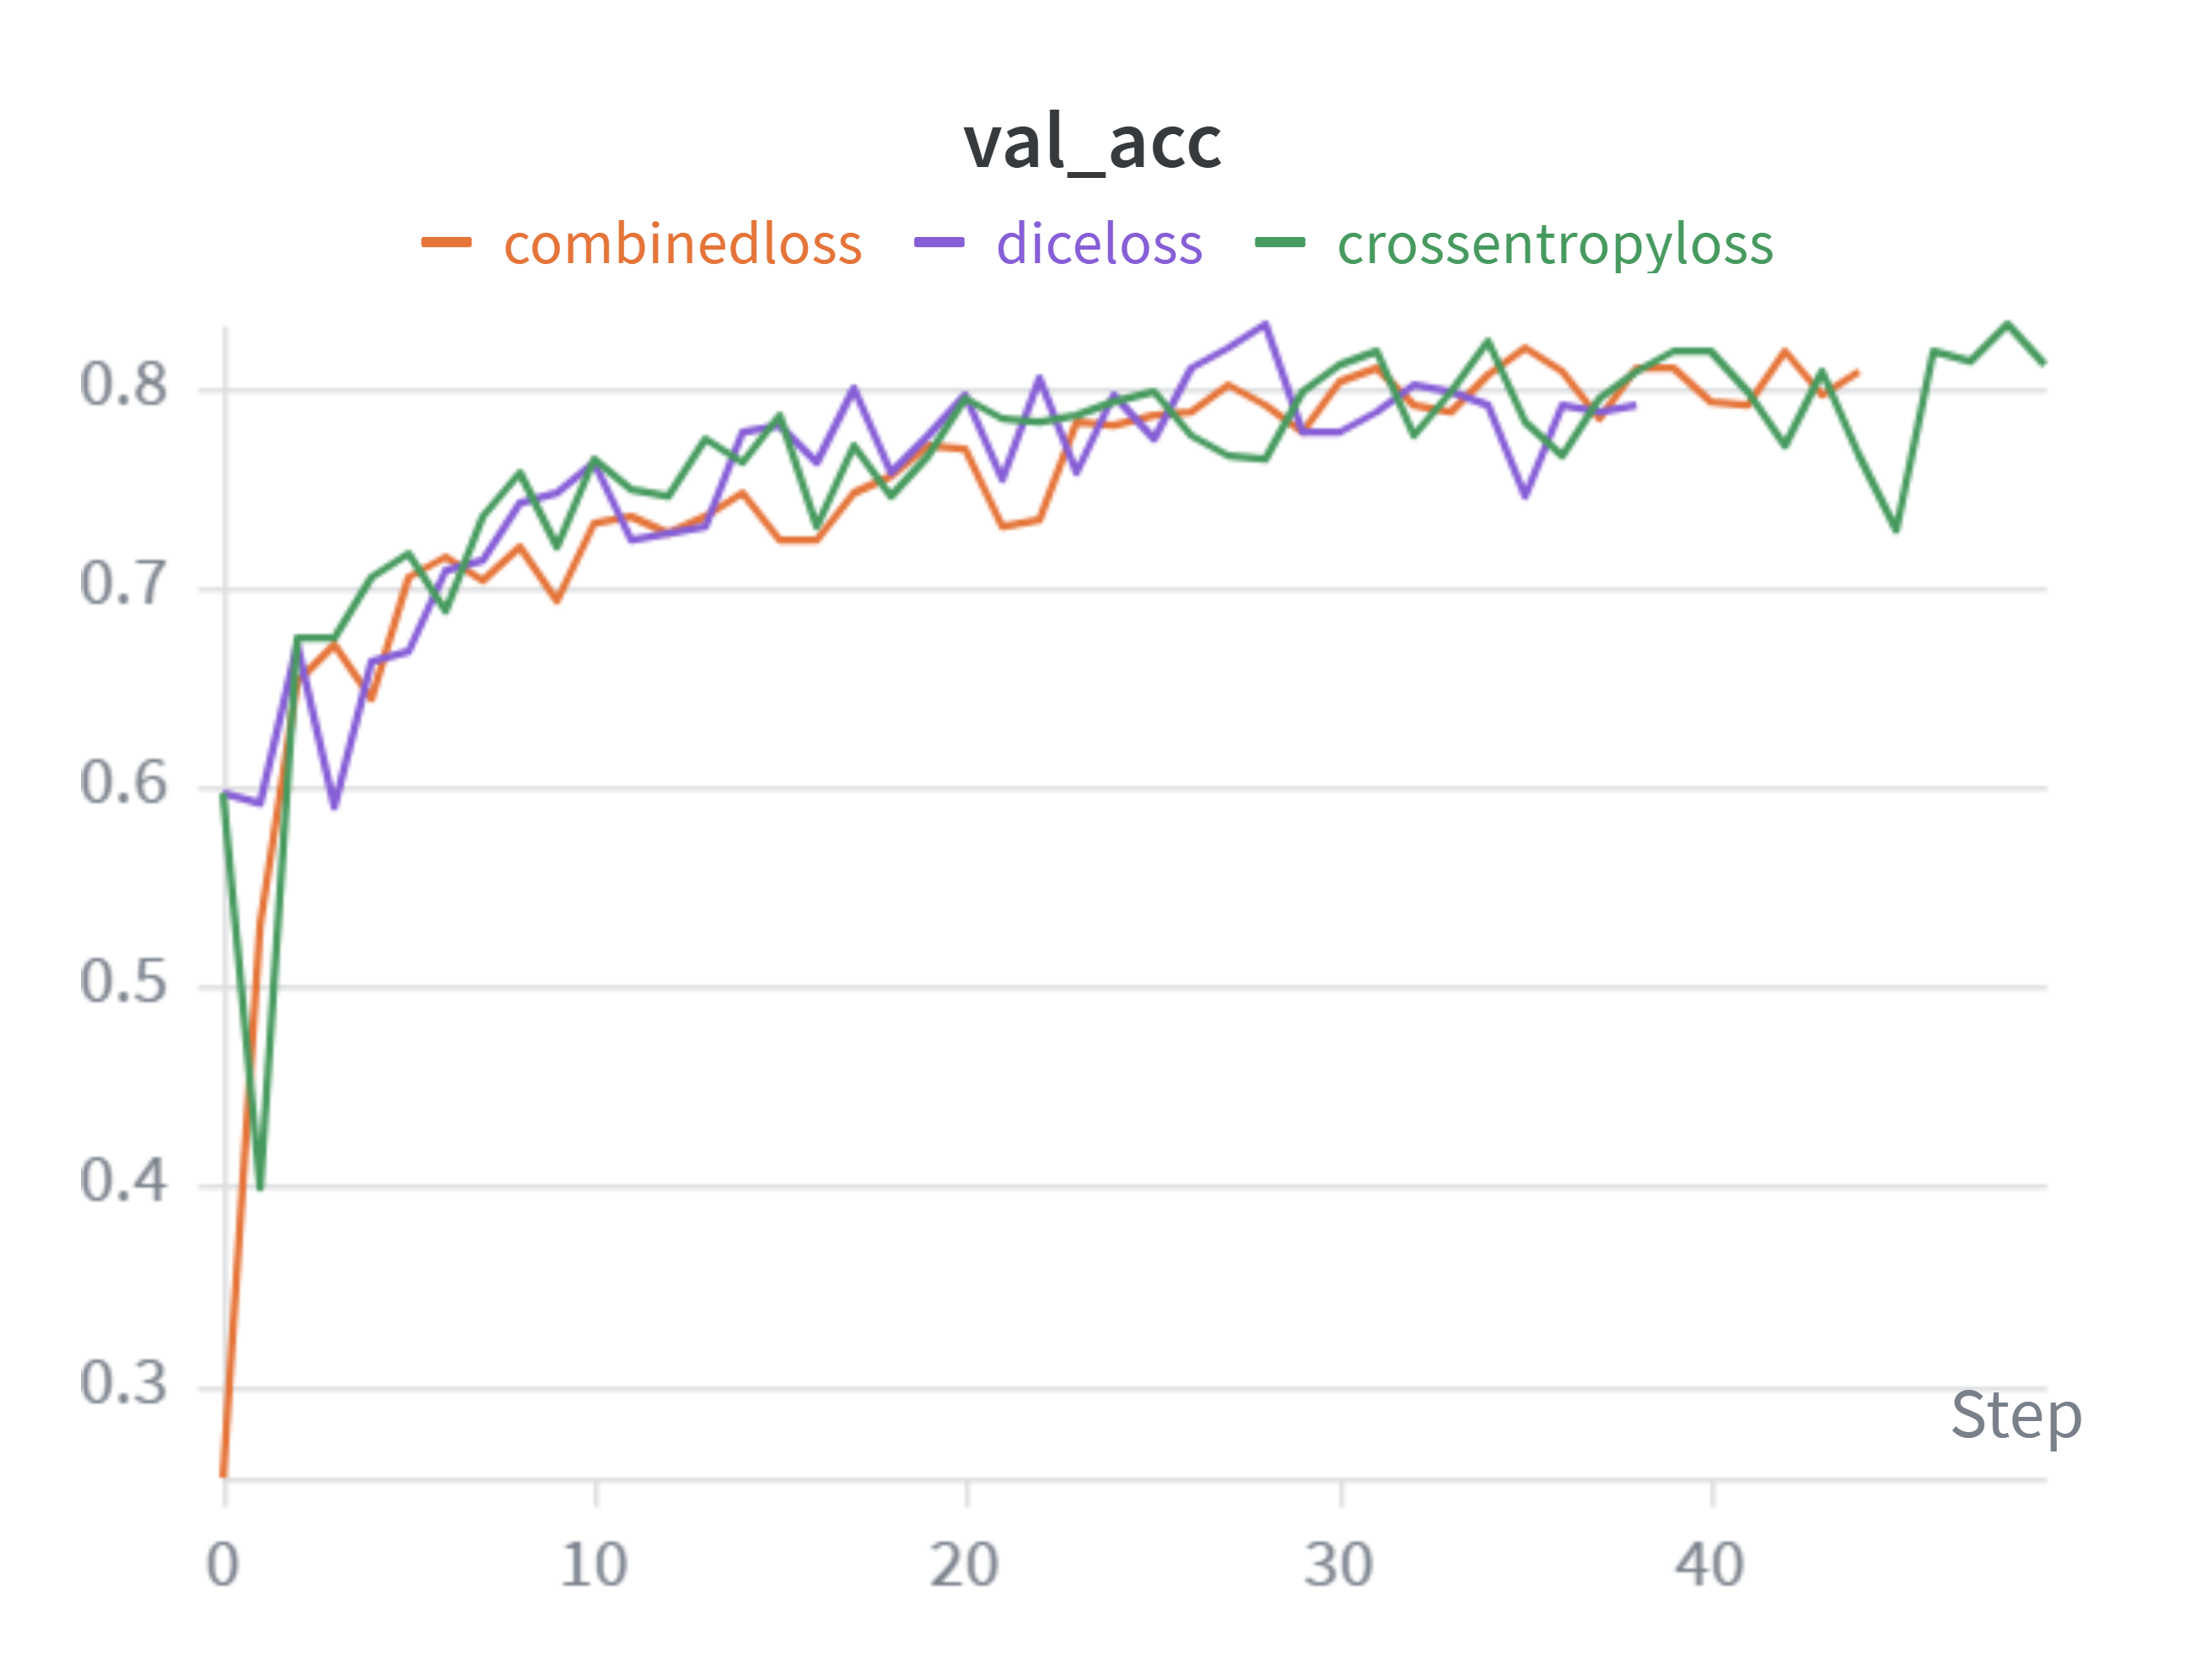
\includegraphics[width=\textwidth]{figures/task3/valaccu.png}
        \caption{Val Accuracy}
        \label{fig:val_acc}
    \end{subfigure}

    \caption{Training and validation metrics over epochs.} % 这里可以替换为你整张大图的主标题
    \label{fig:total_metrics}
\end{figure}
\subsection{Confusion Matrix Analysis}
\begin{figure}[H]
    \centering
    \begin{subfigure}[b]{0.45\textwidth}
        \centering
        
\includegraphics[width=\textwidth]{figures/task3/confusion_matrix.png}
        \caption{Exploratory}
        \label{fig:confusion_matrix1}
    \end{subfigure}
    \hfill
    \begin{subfigure}[b]{0.45\textwidth}
        \centering
        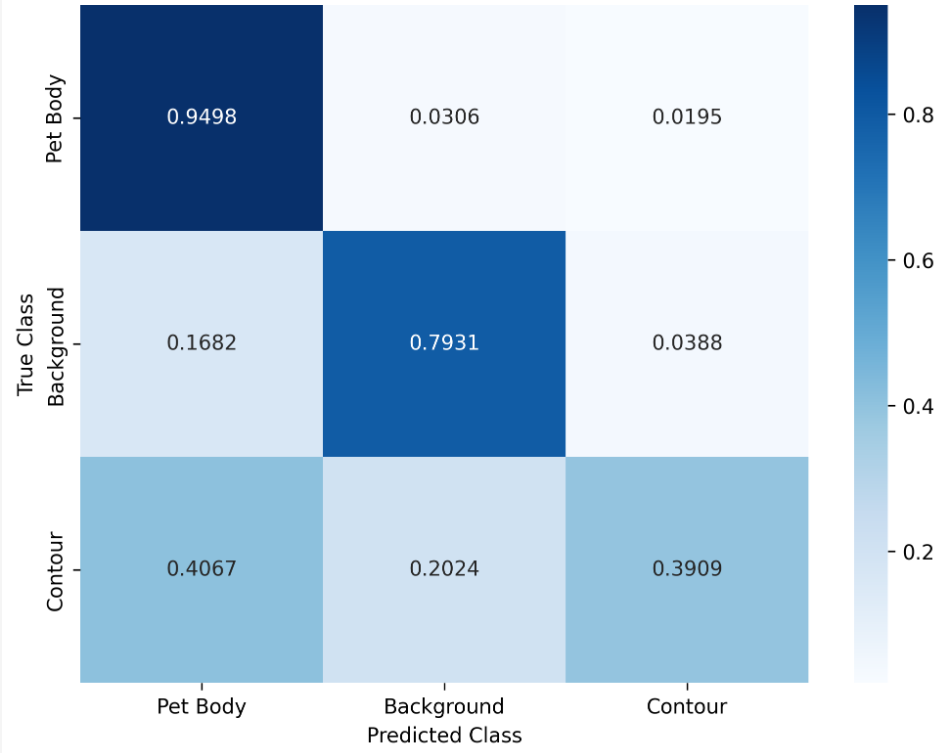
\includegraphics[width=\textwidth]{figures/task3/confusion_matrix2.png}
        \caption{Final}
        \label{fig:confusion_matrix2}
    \end{subfigure}
    \caption{Comparison of confusion matrices for different loss functions.}
    \label{fig:confusion_matrices}
\end{figure}


To further investigate the class-specific performance and understand the granular error patterns across different training scales, a comparative analysis is conducted between the normalized confusion matrices of the exploratory stage (lightweight dataset) and the final stage (full dataset). 

In the exploratory stage, the most frequent confusion pairs include:
\begin{itemize}
    \item \textbf{Contour $\rightarrow$ Background (0.2999):} Approximately 30.0\% of actual boundary pixels are erroneously predicted as background.
    \item \textbf{Contour $\rightarrow$ Pet Body (0.2128):} Around 21.3\% of actual contour pixels are misclassified into the pet's core region.
    \item \textbf{Pet Body $\rightarrow$ Background (0.1718):} About 17.2\% of foreground pet pixels are missed and assigned to the background environment.
\end{itemize}

Upon scaling up to the full dataset in the final stage, a dramatic behavioral shift is observed, where the prominent confusion pairs evolve into:
\begin{itemize}
    \item \textbf{Contour $\rightarrow$ Pet Body (0.4067):} Misclassification nearly doubles, with 40.7\% of boundary pixels engulfed by the pet body.
    \item \textbf{Contour $\rightarrow$ Background (0.2024):} Boundary-to-background drifting decreases to 20.2\%.
    \item \textbf{Background $\rightarrow$ Pet Body (0.1682):} Approximately 16.8\% of true background pixels are falsely detected as foreground pet body.
\end{itemize}

These errors are fundamentally rooted in the spatial ambiguity of the transition region and local visual similarities, but their dynamics change significantly with data scaling. Mechanistically, the \textit{Contour} class represents an extremely thin, line-like structure enclosing the pet. Since boundaries are only a few pixels wide, even a minor spatial shifting or thickness mismatch during U-Net's upsampling phase will drift the predictions into adjacent domains. 

In the exploratory stage, this spatial uncertainty causes the contours to drift almost symmetrically into both background (0.2999) and body (0.2128), yielding a low diagonal accuracy of 0.4873. However, in the final stage, the massive influx of full-dataset training samples drastically strengthens the model's recognition of the foreground, skyrocketing the \textit{Pet Body} diagonal accuracy from 0.7517 to 0.9498. Paradoxically, this dominant foreground representation heavily dilutes the gradient contribution of the sparse boundary pixels. To minimize global loss, the model biases its predictions inward, leading to the "boundary cannibalization" where \textit{Contour $\rightarrow$ Pet Body} surges to 0.4067 and the contour diagonal accuracy collapses to 0.3909. 

Additionally, while the confusion between \textit{Pet Body} and \textit{Background} in the exploratory stage (0.1718) was driven by low-contrast textures like rugs or grass, the final stage introduces a reverse confusion (\textit{Background $\rightarrow$ Pet Body} at 0.1682). This indicates that exposure to highly diverse and cluttered environments forces the final model to occasionally over-segment complex environmental clutters as foreground structures. 

The cross-stage comparison therefore suggests that while the remaining segmentation difficulty is largely caused by the fine-grained edge uncertainty and severe pixel-level class scale variations, the data expansion has successfully resolved the early optimization hurdles of macro-semantic recognition, driving the core target classification to near perfection.
\subsection{Case Analysis}
\begin{figure}[H]
    \centering
    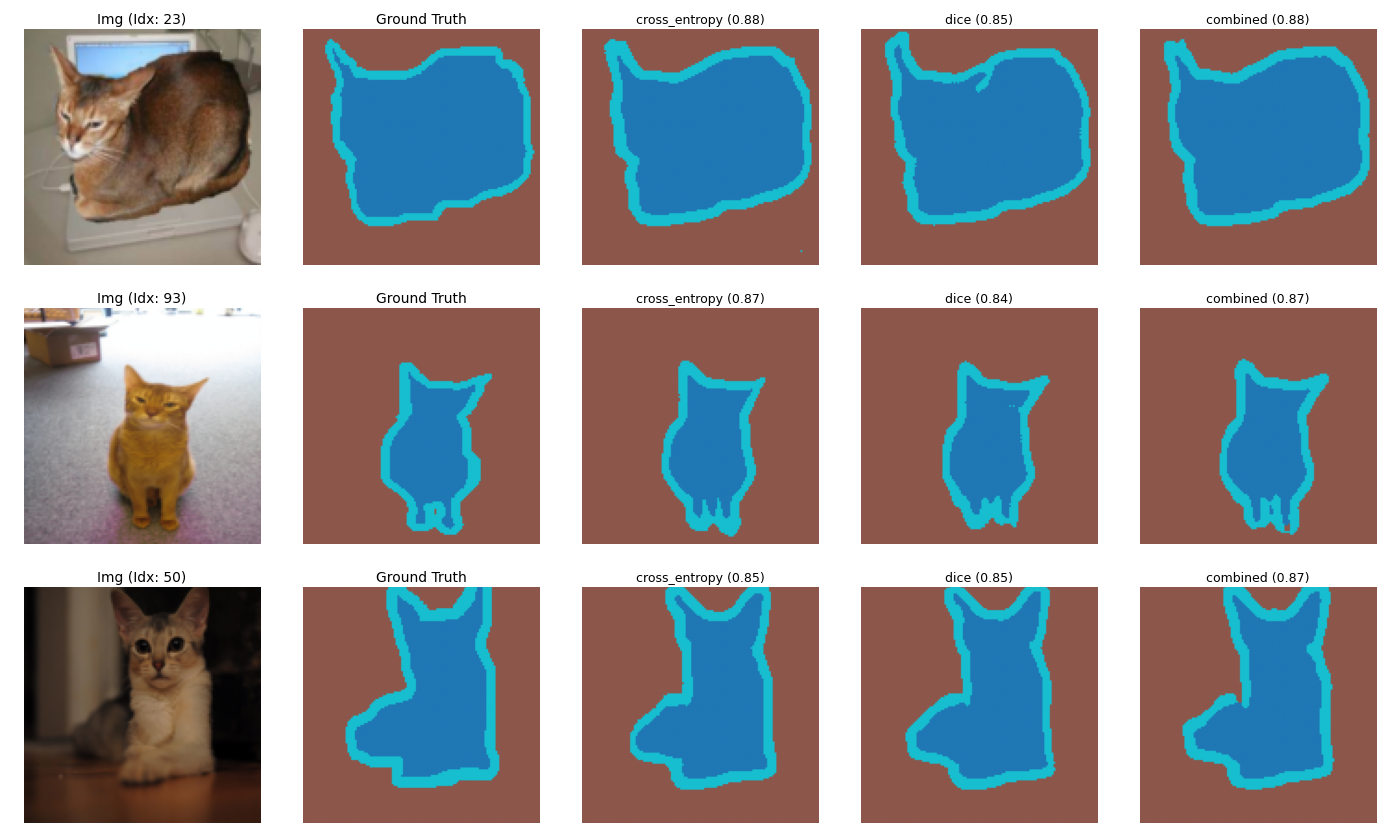
\includegraphics[width=1\textwidth]{figures/task3/comparison.png}
    \label{fig:comparison}
\end{figure}
As observed in Figure(a) (Sample 23), the model demonstrates a remarkable capacity for capturing subtle localized boundaries and leveraging inherent prior features. On the right extremity of the cat's silhouette, the ground truth mask exhibits a subtle omission, failing to meticulously delineate the fine tip of the ear due to localized blurriness. Remarkably, the model optimized with the \textit{Dice Loss} successfully uncovers and encapsulates this delicate structure. This fine-grained segmentation underlines that by directly supervising regional overlap, the \textit{Dice Loss} inherently amplifies the gradient sensitivity toward peripheral boundaries, thereby rectifying minor human annotation omissions and revealing a robust localized structural perception.


In Figure(b) (Sample 93), a distinct challenge emerges within regions subjected to severe environmental illumination and contrast degradation. The narrow spatial gap between the pet's front and hind limbs is characterized by a heavy cast shadow, drastically lowering the pixel-level contrast against the foreground body. The conventional \textit{Cross Entropy Loss} succumbs entirely to this background noise, falsely grouping the shadow domain into the foreground. In contrast, while both the \textit{Dice Loss} and the \textit{Combined Loss} do not fully eradicate this disturbance, they significantly constrain the false-positive area. This phenomenon demonstrates that the integration of region-based constraints helps the encoder suppress localized pixel-level noise by enforcing macro-geometric consistency.

In Figure(c) (Sample 50), the visualization exposes a critical trade-off regarding spatial continuity and topological at complex semantic junctions. While the overall silhouette of the crouching cat is precisely captured, the \textit{Combined Loss} variant unexpectedly introduces a subtle topological fracture—manifesting as a narrow gap or structural discontinuity at the critical intersection where the neck transitions into the forelimbs. Interestingly, both the standalone \textit{Cross Entropy} and \textit{Dice Loss} maintain a continuous, smooth semantic transition in this specific zone. This over-segmentation artifact reveals that during multi-task joint optimization, the intricate gradient dynamics and scaling balance between pixel-wise alignment and regional intersection can occasionally induce localized under-segmentation at structurally non-rigid junctions.
\subsection{Error Case Analysis}
Representative failure cases are shown as follow:

\begin{figure}[H]
    \centering

    \begin{subfigure}{0.8\textwidth}
        \centering
        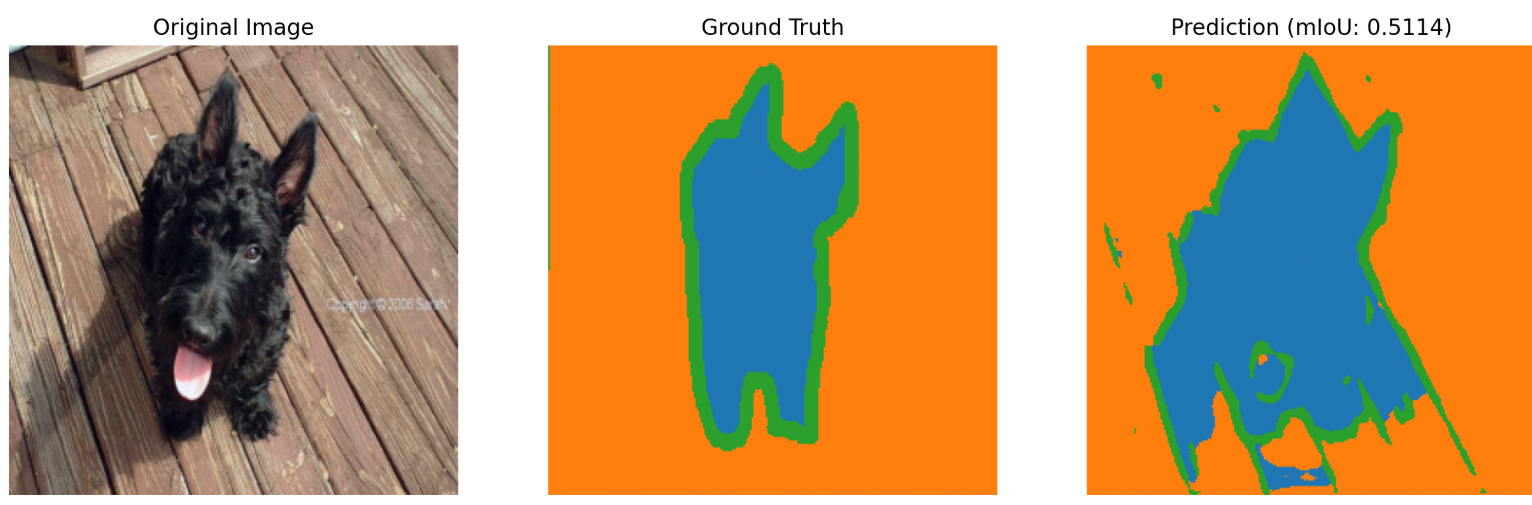
\includegraphics[width=\textwidth]{figures/task3/example7.png}
        \label{fig:case1}
    \end{subfigure}

    \vspace{0.3cm}

    \begin{subfigure}{0.8\textwidth}
        \centering
        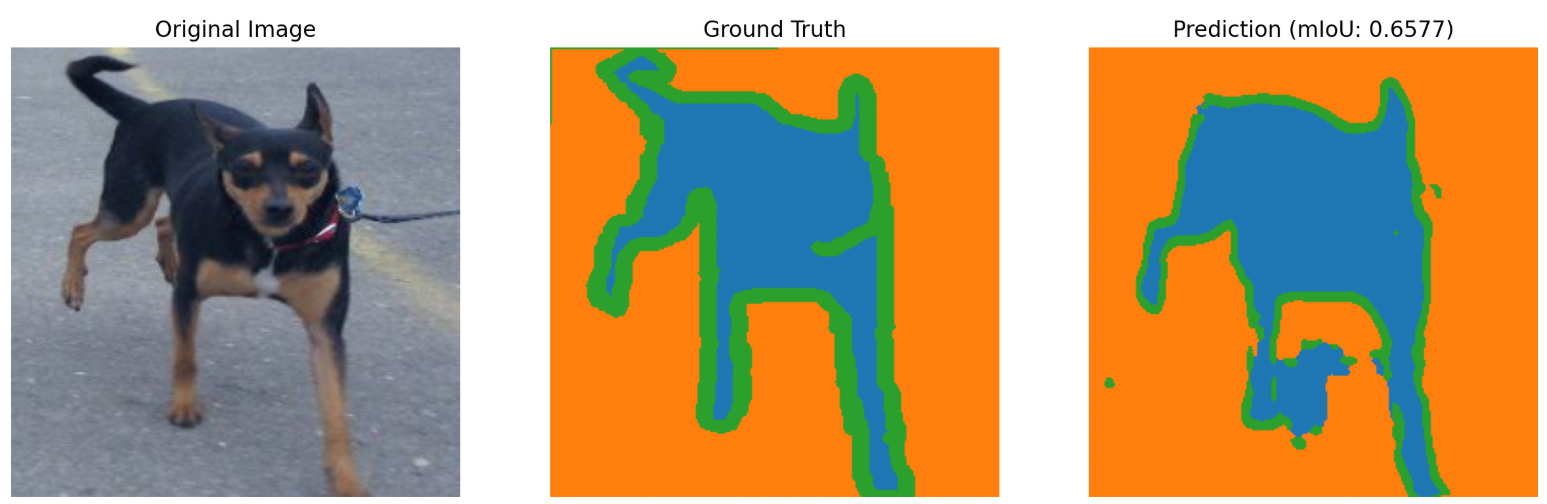
\includegraphics[width=\textwidth]{figures/task3/example5.png}
        \label{fig:case2}
    \end{subfigure}

    \vspace{0.3cm}

    \begin{subfigure}{0.8\textwidth}
        \centering
        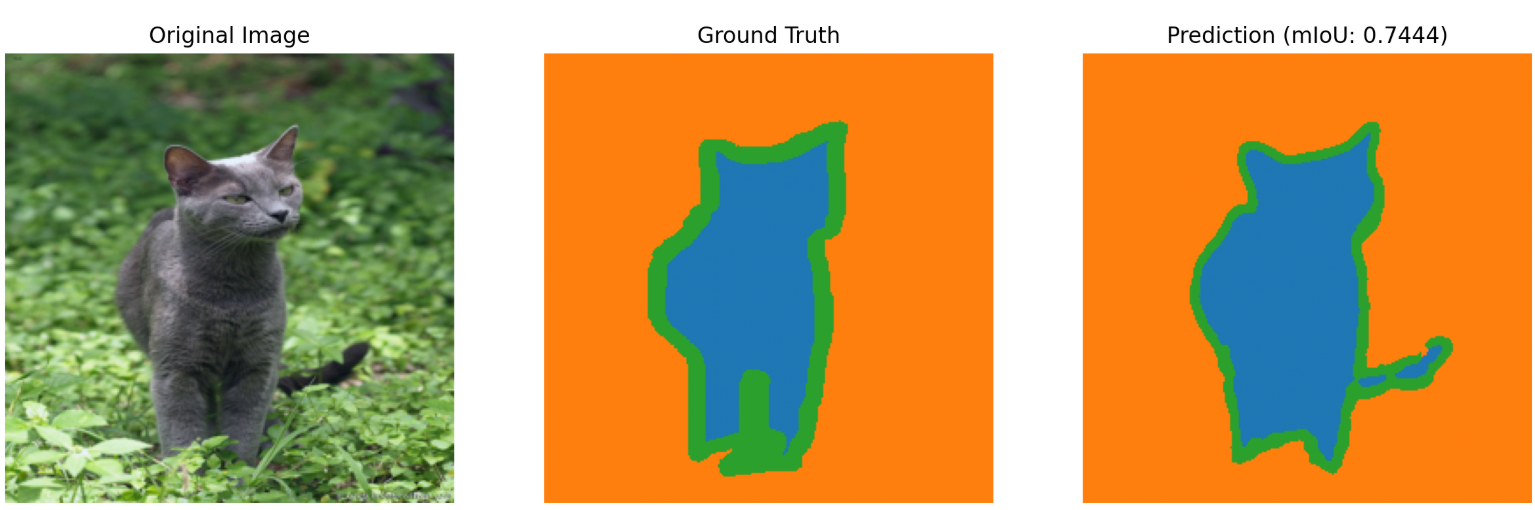
\includegraphics[width=\textwidth]{figures/task3/example6.png}
        \label{fig:case3}
    \end{subfigure}

    \caption{Results comparison}
    \label{fig:all_cases}
\end{figure}


As observed in Figure(a) (Case 1, mIoU: 0.5114), the network experiences extreme spatial distortion when segmenting the black dog on the wooden deck. Chaotic patches of the \textit{Pet Body} class are erroneously generated within the background domain, while the green \textit{Contour} class fractured and expanded unpredictably. This behavior perfectly resonates with the final stage confusion matrix, where 16.82\% of true background pixels are falsely detected as the foreground pet body. Because the model was trained from scratch without pre-trained contextual weights, the highly linear patterns and rich textures of the background wooden planks mimic the geometric complexity of the pet's ears and limbs, causing the encoder to experience local visual illusions.

In Figure(b), a distinctive structural failure occurs at the pet's extremities. While the main trunk of the running dog is segmented near-perfectly, its slender structures—specifically the non-rigid moving legs—suffer from geometric fracturing and semantic drifting. The network fails to sustain a continuous contour around the limbs, leaving the narrow spatial gap under the belly completely misclassified. This highlights that despite the scaled-up training data and the convergence demonstrated in the validation curves, a from-scratch U-Net still struggles with high spatial uncertainty on thin, dynamic appendages due to the pixel-level category scale imbalance where sparse structures provide far fewer gradient updates than bulky bodies.

In Figure(c), the model presents a subtle yet highly instructive detail-level error. The silhouette of the gray cat is captured with exceptional precision, reflecting the high global optimization capacity of the \textit{Combined Loss} and the exceptional 0.9498 diagonal accuracy for the \textit{Pet Body} class. However, the model falsely extends an artificial, slender "tail-like" structure into the right-hand background grass, which does not exist in the ground truth. This over-segmentation reveals the downside of scaling up the training data: as the model becomes overwhelmingly confident in tracking foreground structures, it becomes highly sensitive to linear environmental noise (such as shadows or long blades of grass matching the cat's gray fur tone), misinterpreting them as a continuation of the pet. 

The cross-case visual compilation confirms that while data expansion and the joint loss strategy have successfully driven the core target recognition to near perfection, the fine-grained edge uncertainty and structural boundary vulnerability under cluttered environments remain the primary bottlenecks.